\documentclass[oneside]{book}

\usepackage{fullpage,hyperref,titlesec,enumerate,babelbib,graphicx,float}
\usepackage[english]{babel}
\usepackage{titlesec} % required for removing header spacing

% remove header spacing
\titlespacing\section{0pt}{12pt plus 4pt minus 2pt}{0pt plus 2pt minus 2pt}
\titlespacing\subsection{0pt}{12pt plus 4pt minus 2pt}{0pt plus 2pt minus 2pt}
\titlespacing\subsubsection{0pt}{12pt plus 4pt minus 2pt}{0pt plus 2pt minus 2pt}

% remove all indents
\setlength{\parindent}{0pt}

% Add all chapter folders to graphics path
\graphicspath{
 {./profiling/}
}

\titleformat{\chapter}[hang]{\Huge\bfseries}{\thechapter. }{0pt}{\Huge\bfseries}

\begin{document}
\frontmatter
%%% TITELPAGE %%%

\begin{titlepage}

\begin{center}
\begin{figure}[h!]
\centering
% Title image
% \includegraphics[scale=1]{Images/TU_P2_black.png}
\end{figure}
Faculty of Computer Science \\
\today

\vspace{3.5cm}
\selectfont
{\Large TI3706 - Bachelor Seminar}\\
\vspace{0.0cm}
\Huge{\textbf{Performance Regression Testing\\ A developer's perspective}}
\vspace{0.5cm}
\selectfont

\vspace{5cm}
\normalsize{\textbf{Bachelor Seminar Group}}

\begin{tabular}{ l r}
\normalsize{M.A. Hoppenbrouwer} & \normalsize{4243889} \\
\normalsize{M.J. Otte} & \normalsize{4222695} \\
\normalsize{R.S. Sluis} & \normalsize{4088816} \\
\normalsize{R. Vink} & \normalsize{4233867}\\
\end{tabular}

\vspace{0.75cm}

\begin{tabular}{ l l }
\normalsize{M. Loog} & \normalsize{Professor} \\
\normalsize{C. Bezemer} & \normalsize{Supervisor} \\
\end{tabular}

\end{center}
\end{titlepage}

\chapter{Preface}
In the growing world of tools and methods that are available to a software developer, it becomes harder and harder to keep track of which technique is best to use under what circumstances. This holds true for the growing field of performance regression testing, where new testing strategies are being discovered and discussed, and the steps in the process of detecting performance regressions are being improved constantly. This literature study aims to give an overview of these steps in a way that links each step to a point in the software development process corresponding to the challenges that arise when dealing with performance regression testing in practice.


\chapter{Summary}
% Performance regression testing brings challenges with it. In this paper we discuss what these challenges are, how they are handled and what problems still remain. It shows when it is useful to start performance regression testing during the development. How the data for the tests are gathered. What can be done to process the gathered data. And how to report on it. Ultimately there is still work to be done in the subject, but the paper shows that performance regression testing is a useful method of testing.


\clearpage % To point the bookmark to the top of the page
\pdfbookmark{\contentsname}{toc}
\tableofcontents

\clearpage % To point the bookmark to the top of the page
\pdfbookmark{\listfigurename}{lof}
\listoffigures

% \clearpage % To point the bookmark to the top of the page
% \pdfbookmark{\listtablename}{lot}
% \listoftables

\mainmatter

%  INTRODUCTION
\chapter{Introduction}
\label{chapter:indroduction}
The definition of performance regression testing is: ``Performance regression testing detects performance
regressions in a system under load. Such regressions refer to
situations where software performance degrades compared to
previous releases, although the new version behaves correctly.''\cite{foo2010mining}
Performance regression testing can be seen as the combination of regression testing and performance testing. ``Regression tesing is the retesting of software following modifications.''\cite{rothermel2001prioritizing} Performance testing is testing performance requirements and specifications of it.\cite{gan2006software}

To improve the quality of the software product it could be useful to use performance regression testing in a way the developers can
directly improve the quality of the software product. This will be the main focus of this article. There are different aspects in optimizing performance regression tests, which will be discussed throughout this paper. Every aspect will be clarified in the form of a new chapter in this paper. \\ First of all it needs to be clear how to acquire data and what kind of performance counters will be used for performance regression testing. Next is the filtering of the performance metrics, used to obtain differences in data. The following chapter discusses how to compare the filtered data. Last aspect is that the filtered performance metrics can be reported in the form of visualizations so performance regressions will be detected. At the end of this paper, a research agenda and a conclusion will be provided.


\chapter{organising the testing process}
\label{chapter:organising}
Different methods of software development exist in software engineering. A different type of development means a different way of testing, so it is important to choose a proper development process before a team starts developing. This chapter explains the development methods and how to organise performance regression testing when using each of these methods.

\section{Code-and-fix model}
``The basic model used during the early days of software devolpment contained two steps: write some code and fix the problems in the code'' \cite{boehm1988spiral} This `method' is not appropriate for performance regression testing, because of the poor preparation of testing. It is hard to write test suites without a plan and knowledge of the overall design.

\section{Waterfall method}
``The waterfall method establishes a sequence of stages-requirements, specifications, design, coding, testing and maintenance-to guide the development process. ''\cite{kang1989software}. The sequences of the waterfall method will be done until the development of the system is completed. The waterfall method even became the basis for most software acquisition standards in the past years. \cite{boehm1988spiral}. This type of developing has a testing phase. Collins et al studied an agile waterfall process. \cite{collins2010iterative} A figure giving the phases of the waterfall development process are shown below.

\begin{figure}[H]
\begin{center}
  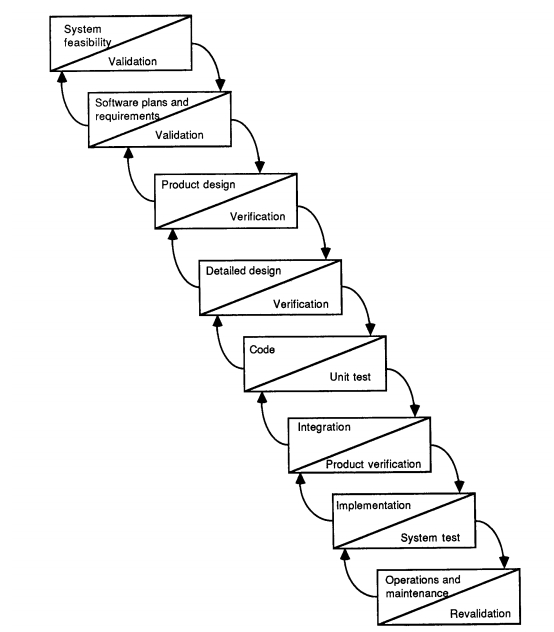
\includegraphics[width=0.5\textwidth]{Figures/waterfall.jpg}
\end{center}
  \caption{Phases during a waterfall development process\cite{boehm1988spiral}} 
\end{figure}

Each rectangle in the figure states as a phase in the waterfall development process. When something goes wrong during the process it will be checked if the errors occurred in the current states. If not, the previous state will be checked. The waterfall method is a static development process. The waterfall method is a static development process. The testing is done near the end of the process, which means that performance regressions are tested near the end of the process too. This suggests that performance regression testing will not be effective, because the tests will be runned when the implementation (almost) done. Although, when using an iterative form of the waterfall method, it can be tested effective. A research showed that, when using an iterative process, regression testing using the waterfall method can be very useful. It even has been stated that most of the time performance is the biggest issue in the field. \cite{foo2010mining} The combination of performance as biggest issue and an effective way of regression testing when using an iterative waterfall process suggests that performance regression testing can be done effective here too.

\section{Spiral method}
``The spiral method creates a risk-driven approach to the software process rather than a primarily document-driven or code-driven process. It incorporates many of the strengths
of other models and resolves many of their
difficulties.''\cite{boehm1988spiral} The phases of the spiral development process are shown in the figure below. 

\begin{figure}[H]
\begin{center}
  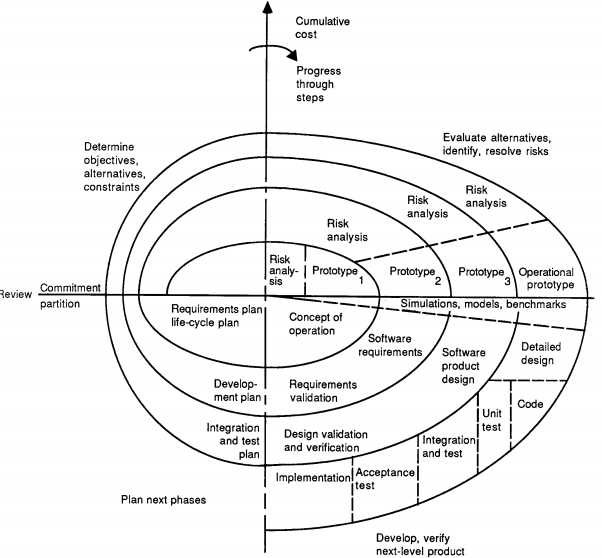
\includegraphics[width=0.5\textwidth]{Figures/spiral.jpg}
\end{center}
  \caption{Phases during a spiral development process\cite{boehm1988spiral}} 
\end{figure}

When using the spiral model, the main focus lies on the different risks of a software project. Examples of these risks are: low budget, developing wrong functions or a continous change of functions. These development processes are divided by the property of their risks. Different prototypes will be made implementing the risks. Performance regression testing can be seen as a risk too, because it can be a demand to maintain the performance when a later prototype is made. This means that the spiral method can be effective when using the spiral method.

\section{Scrum}
``Scrum is an Agile software development process designed to add energy, focus, clarity, and transparency to project teams developing software systems.''\cite{sutherland2007distributed} A Scrum development process is divided into three kinds of phases. Research has been done to show that automated regression tests during the daily builds will greatly improve the quality of the product \cite{Future_of_Scrum}. This means that Scrum is a useful development method for regression testing. When the performance is monitored here as well, the combination of the two can make the testing of performance regressions effective.  \\ There are two organising phases, which are the opening and closing phases. The implementing phase here are the sprints which are further divided. The planning and closing phases are organising phases. It is not necessary to run tests here, because there is either no code (opening) or all the performance regression tests have been executed and passed (closing). Though, planning when to test is an example of an organising aspect which can be done during the opening phase and verifying that the test suite covers all the code can be done during the closing phase. \\ The actual creation of tests will be done during the sprints. The sprints consist of developing, wrapping, reviewing and adjusing. The wrapping part of the sprint, combines all the implemented code. This process of wrapping is a very appropriate moment to test for performance regressions. \\

\section{General aspects of test organization}
Despite the fact that the development method is significant, there are some other organising aspects which could make a difference in the way of performance regression testing. \\
First of all, it can be important who will do the testing. Zaparanuks et al. performed an experiment in which one person did all the testing throughout the project. \cite{sutherland2009fully} This person is an active member of the team and watches all the members of the developing team. This method provides a way to deal with any issues that could come up during the process. The appointed person will directly try to deal with issues coming up by the members of the developing team. By appointing this person, the quality of the product is watched the whole time during the project, instead of comparison to the other research where performance regression testing is done during the merge phase. This experiment indicated that the quality of the development got a much higher average score compared to other similar development products. So appointing one tester who only has the task to watch over the quality by testing and for our sake performing regression tests, can have an improved effect on the overall process. It is not mandatory to use this role division, but it can have a great impact on the performance of the overall product \\

Another organising aspect is to make sure a proper test suite is written before programming, and that this test suite is maintained during the project. This is only done during Test-driven development. ``The test-driven development strategy
requires writing automated tests prior to
developing functional code in small, rapid
iterations.'' \cite{astels2003test} Test suites should be made with some conditions in mind. Writing complete test suites for complex systems will require the regression testing to run for a long time. \cite{rothermel2001prioritizing} So the developers have to decide to either test the complete system, or to write selective test suites. These test suites will only test the main functionality of the system. \\
After deciding the organising aspects, the actual implementation will be initiated. From now on performance regression testing will be done throughout the process. The developers will decide what kind of data of the implementation will be tested. Performance counters can be used to help decide which data the tests will cover.


\chapter{Gathering data}
\label{chapter:gathering}
Once the testing process has been organised to facilitate the particular software development method that is being used, the testing can finally begin. The next challenge that presents itself is what to test for. This chapter discusess what information is relevant to the performance of software and how to handle that information in order to obtain the most accurate representation of the underlying performance.

\subsection{Waterfall method}
``The waterfall method establishes a sequence of stages-requirements, specifications, design, coding, testing and maintenance-to guide the development process. ''\cite{kang1989software}. This method of development even became the basis for most software acquisition standards in the past years. \cite{boehm1988spiral}. The waterfall method can be a good method to test performance regressions. Collins et al researched an iterative waterfall process. \cite{collins2010iterative} The research showed that, when using an iterative process, regression testing using the waterfall method can be very effective. This implicites direclty that performance regression testing will be effective here, because most of the time performance is the biggest issue in the field. \cite{foo2010mining}

\subsection{Spiral metod}
``The spiral method creates a risk-driven approach to the software process rather than a primarily document-driven or code-driven process. It incorporates many of the strengths of other models and resolves many of their difficulties.''\cite{boehm1988spiral} When using the spiral model, the main focus is the different risks of a software project. Examples of these risks are: low budget, developing wrong functions or a continous change of functions. These development processes are divided by the property of their risks. So performance regression testing would not be appropriate for the spiral method, because performance regression tests are not seen as risks.

\subsection{Scrum}
``Scrum is an Agile software development process designed to add energy, focus, clarity, and transparency to project teams developing software systems.''\cite{sutherland2007distributed} A scrum development process is divided into three kind of phases. Research has been done to show that automated regression tests during the daily builds will greatly improve the quality of the product \cite{Future_of_Scrum}. This means that scrum is a useful development method for performance regression testing. \\ There are two organising phases, which are the opening and closing phases and the last phase is the sprint phase which is further divided. The planning and closing phases are organising phases. It is not necessary to run tests here, because there is either no code (opening) or all the performance regression tests have been runned and approved (closing). Though, Planning the test suite is an example of an organising aspect which can be done during the opening phase and verifying that the test suite contains all the tests can be done during the closing phase. \\ The actual implementing will be done during the sprints. The sprints consist of developing, wrapping, reviewing and adjusing. The wrapping part of the sprint, combines all the implemented code. This process of wrapping is a very appropriate way to test for performance regressions.

\section{Types of data: performance counters}
Performance counters are used to measure events that occur duing program execution\cite{PC}. Examples are: the number of instructions, loads, bandwidth or the number of executed cycles.

``The goal of analyzing performance counters is to detect if a performance regression has occured, where the performance regression has occured, and what causes the regression.'' \cite{nguyen2012using}

To detect if performance regressions occur, two different tests will be run: a target run and a baseline run. The target run is the new test run, where the baseline run is a good past run. On both tests equivalent performance counters can be used as input to detect if performance regressiond have occured by comparing the output of the tests. Comparing the output of the tests is a big challenge, especially in big complex software systems.

If it is known that a performance regression has occured, the next problem is to detect where the performance regression has appeared. Big software systems consist of many types of components, and each component may have many instances. Detecting where the perfomance regressions have shown up is very difficult, because there are many performance counters for each instance of each component. This can be very time consuming.

\section{Accuracy and meaning of performance metrics}
After determining the location of the performance regressions, the reason of the performance regressions needs to be determined. ``Understanding the kind of problem usually requires static analysis of source code.'' \cite{nguyen2012using}

The fact that performance counters are often used by application developers shows that performance counters are very useful. However, performance counters ar not that accurate. Tests have shown some factors can increase or decrease the accuracy of performance counters.

For instance, the measurement error possibly increases as the number of registers increases too. However, this is dependent on the counter configuration and the interface used: experiments with two different interfaces and two different counter configurations show different results, and for only one of the four ombinations of the interface and counter configuration the measurement error increases. \cite{AccuracyPerforanceCounter} So most of the times the number of registers doesn't matter.

Also, the type of infrastructure is very dependent. The measurement error reduces a lot when a low-level infrastructure is used, instead of a high-level infrastructure. \cite{AccuracyPerformanceCounter}

On top of that, for the user+kernel mode the measurement error gets bigger if the duration of the benchmark gets longer. \cite{AccuracyPerformanceCounter} So to make the measurement error smaller, less loop iterations should be used.  For the user mode the duration of the benchmark does not matter. This is because of interrupts, that only occur in kernel event counts. More interrupt-related instructions will include if the duration of a measurement takes longer.


\chapter{Data filtering}
\label{chapter:filtering}
\section{Control charts}
Detecting if performance regression has occured manually costs a lot of time. Comparing each performance counter with a prior good test is a lot of work. A possible way to analyze the results faster is to use a control chart.
``The goal of control charts is to automatically determine if a deviation in a process is due to common causes, e.g., input fluctuation, or due to special causes, e.g., defects'' \cite{nguyen2012using}. Control charts are often used to detect problems in manufacturing processes where raw materials are inputs and the completed products are outputs. An example of a control chart can be seen in figure 4.1. \

\begin{figure}[h]
\begin{center}
  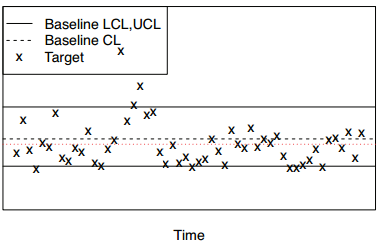
\includegraphics[scale=0.7]{Figures/controlchart.png}
\end{center}
  \caption{from ``Example of a control chart''\cite{nguyen2012using}}

\end{figure}


A control chart consists of a baseline data set (CL) and a target data set (Target). A baseline data set contains the results of the prior test. Based on this data set an upper (UCL) and lower limit (LCL) will be decided. The target data set contains the results of the new test.

From these two data sets the violation ratio can be calculated. This is the percentage of the amount of targets outside the upper and lower limit. If performance regression occurs, the violation ratio is too high. In figure 1 only a few targets are outside the upper and lower limit, so most probably no regression has occured.

It now seems easy to detect if performance regression occurs: a certain threshold on the maximum allowed violation ratio can be chosen, and if the violation ratio is higher than this threshold, performance regression has occurred. Unfortunately, this is not the case. There are some reasons that make it hard to detect performance regression. If the violation ratio is low, the probability that performance regression has occurred is low as well. A high violation ratio doesn't always mean that performance regression has occurred. Some performance counters are inconsistent, and show different results on the same input data. Because of this, it is possible that the violation ratio is higher than the chosen threshold but no performance regression has occurred. To avoid this, the prior test will be executed again after the new test.

\section{Association rules}
Another way to filter the results of performance regression testing is by using association rules. An association rule has a premise and a consequent. A rule predicts the occurence of a consequent, based on a premise. Association rules can be derived from a frequent item set. ``A frequent item set describes a set of metrics that appear together frequently''\cite{foo2010mining}. To discover a frequent item set, the Apriori algorithm can be used. The Apriori algorithm uses support and confidence to reduce the amount of candidate rules generated:
``Support is the frequency at which all items in an association rule are observed together'' \cite{foo2010mining}. If the support is low, the assocation should not be analyzed, but if the support is high it should. Confidence is the probability that the assocation rule's premise leads to the consequent and has a value between 0 and 1. If the value is 0, it means that the confidence has not changed for a new test, and if the value is 1 the confidence of a rule is totally different. A threshold is created to filter out the consequences of the rules that have changed to much.








\chapter{Comparing results}
\label{chapter:comparing}
Even though filtering test results can greatly reduce the amount of data that is involved in analyzing testing results, in order to detect performance regressions the results still have to be compared in some way to the results of a previous run of the test suite. The following are some of the problems that arise when doing so and some of the solutions that exist.

\section{Load-independent comparison}
Performance metrics are dependent on the system load during execution of the test suite. This makes it difficult to correctly identify performance regressions. Jiang et al present an automated way to abstract load testing data and analyze the behaviour of the system. \cite{jiang2010automated} Even though it is not intented to be used for performance regression testing specifically, it uses performance counters to compare system performance to predefined criteria and as such present a solution to the load dependency of performance counters.

Model based testing leverages the advantage of being load-independent against the tasks of having to keep the model up-to-date. The load-independence also only goes as far as the different load for which the model was solved, which means it is not a viable method for detecting performance regressions when system load behaves in ways that was not anticipated in advance. Mi et al offer a way to derive a performance signature that is based on the latency of a transaction and the utilization of system resources, which are adjusted for the existence of outliers \cite{mi2008analysis}.

\section{Detecting possible performance regressions}
In order to detect performance regressions in a system, a method of comparing the performance of different versions of the system is required. Since manual comparison is prone to errors and not viable for large amounts of performance metrics, the method should be able to automatically compare the performance by creating a profile for a version of the software and comparing it with the profile of previous verions. There are different ways to do this and they are likely to yield different results.

By normalizing and discretizing the performance counters and correlating the results against a historal dataset Foo et al are able to derive a perforance signature \cite{foo2010mining} consisting of association rules between performance counters. An example of such a signature could be \{Arrival Rate = Medium, CPU utilization = Medium, Throughput = Medium\}. In combination with statistical techniques, these association rules enable analysts to automatically flag violations of rules in new tests and detect possible performance regressions with a certain confidence.

\section{Tracing the cause of performance problems}
Tracing the cause of anomalies in performance can help in indentifying if something is a performance regression and what might have caused it. There are several approaches that aim to identify the underlying cause of performance regressions.

If the performance metrics measure system level activity, it is difficult to trace a performance regression back to the function call that causes it. By probing I/O write operations on application level, Bezemer et al are able to create a profile for the amount of I/O per function \cite{bezemer2014detecting}. This allows them to trace performance problems back to changes in specific function by comparing performance metrics with the version control system of the tested software. Not only does this provide the cause of the problem, it enables developers to use performance regression testing to guide optimizing performance.

Ghaith et al build on the principle of load-independent and model based testing by using a queueing network to model the underlying system and using historical testing data to tune the model to the expected performance under various workloads. \cite{ghaith2013profile} This approach combines a transaction profile, a signature of the system resources utilized by some elementary action of the system, with historical testing data. A transaction profile can be obtained using statistical techniques for determing the service demands based on resource utilization \cite{casale2008robust} or response time \cite{kraft2009estimating}.


\chapter{Reporting and drawing conclusions}
\label{chapter:reporting}
After acquiring, filtering and comparing the data, the metrics can be reported. The following chapter will show the reporting of the results of performance regression testing. It will touch on visualization and dectection of the performance regressions. \newline
\newline
As mentioned in chapter 2, the choice of performance metric is very important. When making a report, this is what it will be based around. A report based on cpu time will have a different structure than a report based on bandwith. The performance metrics require additional data to be able to show regressions. This additional data can be number of times the performance regression test has been executed or the number of times a particular function has been called. This kind of data can be useful to determine if a performance regression has occured. If due to a new functionality a function is expected to be called twice as much since the last revision, an increase in performance can be expected.\newline

\section{Visualization}
When a report is created, a large amount of data can be useful. Only it is very hard and error sensitive to look over those numbers. Visualization can be used to show the data in a way that might be easier to comprehend. By using visual representations such as a graph, will make it easier to spot a change in revisions.

\section{detection of performance regressions}





%mogelijk report techniek: transaction profile
%http://onlinelibrary.wiley.com/doi/10.1002/stvr.1573/pdf
%average precision and recall
%http://sail.cs.queensu.ca/publications/pubs/qsic2010_foo.pdf


\chapter{Research agenda}
\label{chapter:agenda}
Spanning the years and the papers that have been discussed in this report, a lot of problems and possible solutions are introduced. This section provides an overview of the problems and solution per paper, as well as a list of problems that are yet to be solved.\\

Performance regression testing and load testing share the dependency of results on the system load and the problem of detecting performance problems. Jiang et al propose an automated approach to detect functional and performance problems that scales well to enterprise systems and provides high precision results \cite{jiang2010automated}. It can be used to analyze the behavior of a system during a load test, and with regards to performance regression testing, to abstract over the load testing data, allowing for load-independent conclusions to be drawn.

Analyzing load tests results to detect performance regression is
very time consuming due to the large amount of performance
counters. Nguyen et al propose an approach that uses control charts, a statistical process control technique. to assist performance engineers in identifying test runs with performance regressions, pinpointing the components which cause the regressions, and determining the causes of regressions in load tests \cite{nguyen2012using}.

Client-server applications are widespread nowadays. Understanding the cascading effects of the various tasks that are sprung by a single request-reply transaction is a challenging task. Kraft et al address the issue of efficiently diagnosing essential performance changes in application behavior in order to provide timely feedback to  application designers and service providers \cite{kraft2009estimating}. They propose a new approach based on an application signature built on the concept of transaction latency profiles and transaction signatures. The approach is non-intrusive and based on monotoring data that is typically available in enterprise applications.

Transaction profiling using larger deployments contains a local optimum which not have been experimented with, a plan to use different search techniques could be a possible research for the future. \cite{ghaith2013profile} Transaction profiles from output load runs, which include the response time and resource utilization only works in simple deployments, due to single node assumption they require multiple runs with multiple load. This means that the time spent on testing with the use of transaction profiling can take a long time.

When using a transaction profile, the amount of data that populates the database can have an affect on the profile. This data can mainly affect the database CPU and I/O. \cite{ghaith2015anomaly}

In Chapter 3 a I/O gathering method is explained. This method uses a considerable amount of overhead. Thus the use of time sensitive metrics is unreliable. \cite{bezemer2014detecting}

The identification of performance regressions can be hard. \cite{foo2010mining} Service Level Objectives are used to determine if anomalies have occurred, but Service Level Objectives are not used very often. Identifying performance regressions manually can be subjective. Individual analists can overlook some important performance metrics. Automated identification can be hard as well, because there could be phase shifts in the performance tests, spikes can be different for each test. This will make it hard to use classifier techniques.

The filtering technique used in the paper did not measure some performance regressions. It only used the Apriori algorithm, where other filtering can be necessary to detect undefined performance regressions.

If performance regressions are in the in the system from the start of the development, it will not be detected.



% CONCLUSION
\newpage

\chapter{Conclusion}
\label{chapter:agenda}
This paper shows that performance regression testing could help the developer improve their system. To do so the developer needs to gather performance metrics, process this data and draw meaningful conclusions from it. If all these steps are made, the developer can tell what kind of performance regressions have occurred, so they can adjust their system. Performance regression testing is a rather new subject in the field Computer Science. This means that it can be further investigated. Some of these future experiments can be found in the research agenda.


% Appendices
% \appendix

% END appendices

\backmatter

\phantomsection
\addcontentsline{toc}{chapter}{\bibname}

\bibliographystyle{unsrt}
\bibliography{bibliography}

\end{document}
